%
% File emnlp2018.tex
%
%% Based on the style files for EMNLP 2018, which were
%% Based on the style files for ACL 2018, which were
%% Based on the style files for ACL-2015, with some improvements
%%  taken from the NAACL-2016 style
%% Based on the style files for ACL-2014, which were, in turn,
%% based on ACL-2013, ACL-2012, ACL-2011, ACL-2010, ACL-IJCNLP-2009,
%% EACL-2009, IJCNLP-2008...
%% Based on the style files for EACL 2006 by
%%e.agirre@ehu.es or Sergi.Balari@uab.es
%% and that of ACL 08 by Joakim Nivre and Noah Smith

\documentclass[11pt,a4paper]{article}
\usepackage[hyperref]{emnlp2018}
\usepackage{times}
\usepackage{latexsym}
\usepackage{url}
\usepackage{amsmath}
\usepackage{algorithm}
\usepackage{algorithmic}
%%% YOUR PACKAGES BELOW THIS LINE %%%
\usepackage[small,bf]{caption} % added MLF 20171211
\usepackage{multicol}
\usepackage{adjustbox}
\usepackage{graphicx}
\usepackage{array,multirow}

%\aclfinalcopy % Uncomment this line for the final submission

\setlength\titlebox{5cm}
% You can expand the titlebox if you need extra space
% to show all the authors. Please do not make the titlebox
% smaller than 5cm (the original size); we will check this
% in the camera-ready version and ask you to change it back.

\newcommand\BibTeX{B{\sc ib}\TeX}
\newcommand\confname{EMNLP 2018}
\newcommand\conforg{SIGDAT}

\title{Fixing Translation Divergences in Parallel Corpora for Neural MT}
%\title{A Recurrent Network for Parallel Corpora Divergence Analysis}

\author{%Minh Pham, \ Fran\c cois Yvon\\
  First author\\
  Affiliation / Address line 1\\
  Affiliation / Address line 2\\
  Affiliation / Address line 3\\
  {\tt email@domain}  
  \And
  %Josep Crego, \ Jean Senellart\\
  Second author\\
  Affiliation / Address line 1\\
  Affiliation / Address line 2\\
  Affiliation / Address line 3\\
  {\tt email@domain}}

\date{}

\begin{document}
\maketitle
\begin{abstract}

%http://www.airccj.org/CSCP/vol4/csit42503.pdf

Corpus-based approaches to machine translation rely on the availability of parallel corpora.
%and their performance is highly linked to the quality of the parallel data. 
According to the process followed to compile a parallel corpus, it may contain multiple parallel sentences that are often not as parallel as one might assume. 
%Examples are easily found when corpora is created from non-parallel texts or included by noisy document/sentence alignment tools.
This paper describes an unsupervised method for detecting translation divergences in parallel sentences. 
%We use a deep neural network to predict word alignment scores in parallel sentences. 
We present a neural network to predict sentence similarity that minimises a loss function based on word alignments.
We show that accurate predictions are obtained allowing divergent sentences to be filtered out. 
Furthermore, word similarity scores predicted by the network are used to identify and fix some divergences guiding to more parallel segments.
%Misaligned words are then identified allowing divergent parallel sentences to be filtered out and in some cases making sentences parallel by removing such words. 
We evaluate the presented method on an English-French and an English-German machine translation tasks. 
Results show that neural MT systems trained on the filtered/corrected corpus outperform the MT systems trained on the original data.
%This method can be used on any parallel corpus without any manual annotation.

\end{abstract}

\section{Introduction}

Parallel sentence pairs are the only necessary resource to build Machine Translation (MT) systems. 
In the case of Neural MT, a large neural network is trained through maximising translation performance on a given parallel corpus. 
Therefore, the quality of an MT engine is heavily dependent upon the amount and quality of parallel sentences. 
Unfortunately, parallel texts are scarce resources. 
There are relatively few language pairs for which parallel corpora of reasonable sizes are available, and even for those pairs, the corpora come mostly from few domains. 
To alleviate the lack of parallel data several approaches have been developed in the last years. 
They range from methods using non-parallel, or comparable data ~\cite{Zhao:2002:APS:844380.844785,W04-3208,J05-4003,W17-2509,P17-3003} to techniques that produce synthetic parallel data from monolingual corpora ~\cite{P16-1009,W17-4714} using in all cases automated alignment/translation engines that are prone to the introduction of noise in the resulting parallel sentences. 
Mismatches on parallel sentences extracted from translated texts are also reported ~\cite{tiedemann2011bitext,XU16.310}. 
This problem is mostly ignored in machine translation, where parallel sentences are considered to convey the exact same meaning, and is particularly important for neural MT engines as suggested by~\cite{chen2016adaptation}.

Table~\ref{tab:examples} illustrates some examples of English-French parallel sentences which are not completely semantically equivalent. Examples are extracted from the OpenSubtitles corpus~\cite{LisonTiedemann2016}. 
Divergences are outlined using bold letters. 
Additional segments are included on either side of the parallel sentences (first and second rows). 
Some translations may be completely uncorrelated (third row) or inaccurate (fourth row).
Note that divergent translations are due to many different reasons ~\cite{C14-1055}, the study of which is beyond the scope of this paper.

\begin{table}[ht]
\small
\center
\begin{tabular}{ c|l }
  \hline  
  \texttt{en} & \it{What do you feel}\bf{, Spock}\it{?} \\
  \texttt{fr} & \it{Que ressentez-vous?} \\
  \texttt{gl} & {\small \it{What do you feel?}} \\
  \hline
  \texttt{en} & \it{How much do you get paid?} \\
  \texttt{fr} & \it{T'es pay\'e combien} \bf{de l'heure}\it{?} \\
  \texttt{gl} & {\small \it{How much do you get paid per hour?}} \\
  \hline  
  \texttt{en} &  \bf{That seems a lot.} \\
  \texttt{fr} & \bf{40 livres?} \\
  \texttt{gl} & {\small \it{40 pounds?}} \\
  \hline  
  \texttt{en} & \it{I brought you} \bf{french fries}\it{!} \\
  \texttt{fr} & \it{Je t'ai rapport\'e des} \bf{saucisses}\it{!} \\
  \texttt{gl} & {\small \it{I brought you sausage!}} \\
  \hline
\end{tabular}
\caption[Table caption text]{Examples of semantically divergent parallel sentences. English (\texttt{en}), French (\texttt{fr}) and gloss of French (\texttt{gl}). }
\label{tab:examples}
\end{table}

In this work, we present a neural divergence classifier aimed at detecting words on either side of parallel sentences for which the corresponding meaning is not present on the translated counterpart. 
We evaluate the classifier on an English-French and an English-German translation tasks showing that translation accuracy can be improved by filtering out divergent sentence pairs.
In addition, we  show that some divergent sentences can be fixed by removing divergent words, further boosting translation accuracy. 

The remainder of this paper is structured as follows. Section~\ref{related} overviews related work. 
We describe in detail the core of the neural divergence classifier and the correction algorithm in Section~\ref{sec:divergence}. 
Section~\ref{experiments} details the experiments conducted to measure the ability of the presented classifier to identify and fix divergent sentences.
Section~\ref{sec:results} evaluates results. 
Finally, conclusions are drawn in Section~\ref{conclusions} while further work is outlined in Section~\ref{further}.
All the code used in this paper as well as a human annotated test set are freely available\footnote{\texttt{https://github.com/anonymised}}.

\section{Related Work}
\label{related}

Attempts to measure the impact of translation divergences in MT systems have focused on the introduction of noise in sentence alignments ~\cite{goute2012}, showing that statistical MT systems are highly tolerant to noise, and that performance only degrades seriously at very high noise levels. 
In constrast, neural MT engines seem to be more sensitive~\cite{chen2016adaptation}, as they tend to assign high probabilities to rare events~\cite{Hassan2018AchievingHP}.

Efforts have been devoted to characterise the degree of semantic equivalence between two snippets of text in the same or different languages~\cite{conf/semeval/AgirreBCDGMRW16}, a workshop devoted to an objective similar to our work. 
In~\cite{Mueller:2016:SRA:3016100.3016291}, a monolingual sentence similarity network is proposed, making use of a simple LSTM layer to compute sentence representations. 
The authors show that a simple SVM classifier can be built on top of the sentence representations to achieve state-of-the-art results in a semantic entailment classification task. 
With the same objective, the system presented in~\cite{N16-1108} uses multiple convolutional layers and models pairwise word interactions. %Our work differs from the previous as we build a different network and use it to measure similarity of sentences in different languages. 

Our work is inspired by~\cite{W17-3209} where the authors train a cross-lingual divergence detector using word alignments and sentence length features to train a linear SVM classifier. 
Their work shows that an NMT system trained only on non-divergent sentences yields slightly higher translation quality scores and requires clearly less training time. 
The same authors have recently updated their work in~\cite{DBLP:journals/corr/abs-1803-11112}. 
The objective is the same as the neural network presented in~\cite{N16-1108} and their network further outperforms their previous work. 
Our work differs from the previous as we make use of a network with different topology. 
We model sentence similarity by means of optimising a loss function based on word alignments. 
Furthermore, the network predicts word similarity scores that we further use to correct divergent sentences.

\section{Neural Divergence Classifier}
\label{sec:divergence}

The architecture of our model is inspired by the work on Word Alignment in~\cite{W16-2207}. Figure~\ref{network} illustrates the model.

\begin{figure}[h]
\center
    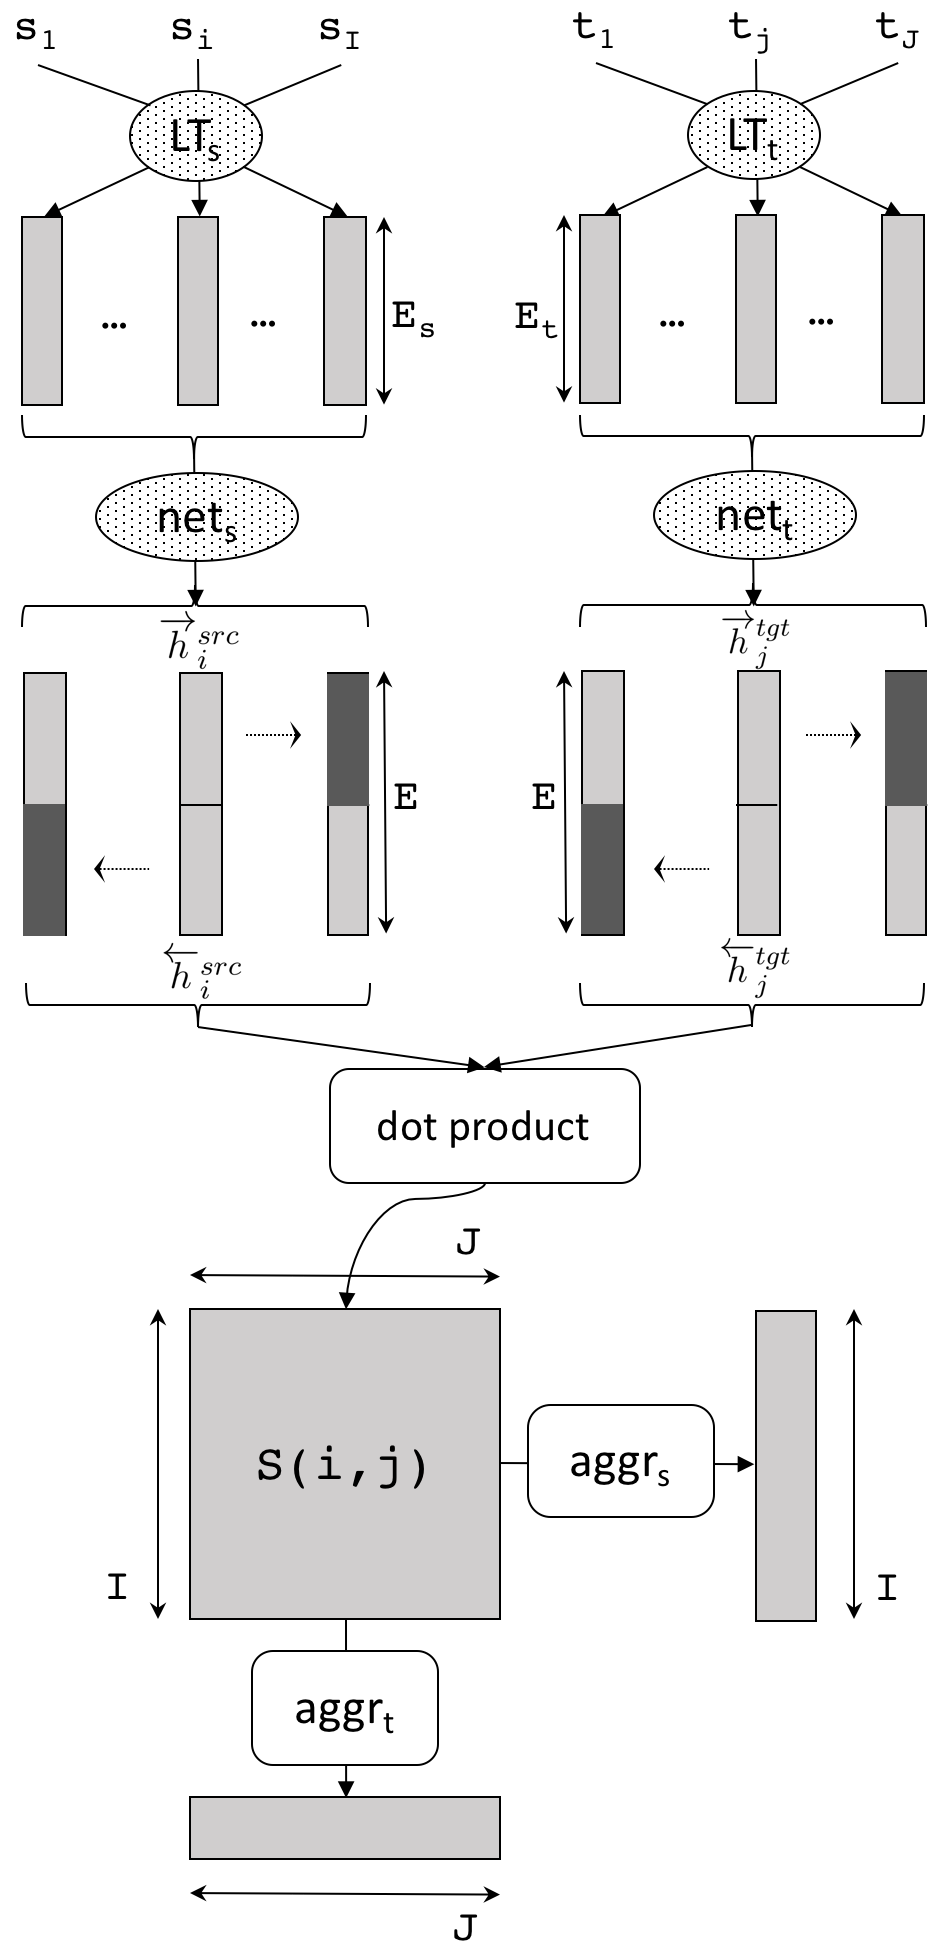
\includegraphics[width=0.8\linewidth]{network}
    \caption{Illustration of the model.} 
    \label{network}
\end{figure}
 
%\subsection{Divergence Network}

In the following, we consider a source-target sentence pair $(s,t)$ with $s=(s_1,...,s_I)$ and $t=(t_1,...,t_J)$. 
The model is composed of 2 Bi-directional LSTM subnetworks, $net_s$ and $net_t$, which respectively encode source and target sentences. 
Since both $net_s$ and $net_t$ take the same form we describe only the source architecture.

The source-sentence Bi-LSTM network outputs forward and backward hidden states, $\overrightarrow{h}^{src}_i$ and $\overleftarrow{h}^{src}_i$, which are then concatenated into a single vector encoding the $i^{th}$ word of the source sentence, 
$h^{src}_i = [ \overrightarrow{h}^{src}_i ; \overleftarrow{h}^{src}_i ]$.
In addition, the last forward/backward hidden states (outlined using dark grey in Figure~\ref{network}) are also concatenated into a single vector  to represent whole sentences 
$h_{src} = [ \overrightarrow{h}^{src}_I ; \overleftarrow{h}^{src}_1 ]$.
At this point, a measure of similarity between sentence pairs can be obtained by cosine similarity:
\begin{equation}
    sim(h_{src}, h_{tgt}) = \frac{h_{src} \cdotp h_{tgt}}{||h_{src}|| * ||h_{tgt}||}
    \label{cosine}
\end{equation}
%\noindent where two vectors (embeddings) with the same orientation have a cosine similarity of $1$, while two vectors with opposed orientation have a similarity of $-1$, independent of their magnitude.

Our model can be optimised following two different objective functions:

\begin{description}
    \item[wemb] 
 
Maximise the word alignment scores between words of both sentences using aggregation functions that summarise the alignment scores for each source/target word. 
Similar to~\cite{W16-2207} alignment scores $s(i,j)$ are given by the dot-product $S(i,j) = h_i^{src} \cdotp h_j^{tgt}$, while aggregation functions are defined as:   
\begin{equation}
\begin{split}
    aggr_s(i,S) = \frac{1}{r} \ log \left( \displaystyle \sum_{j=1}^{J} e^{r * S(i,j)}\right) \\
    aggr_t(j,S) = \frac{1}{r} \ log \left( \displaystyle \sum_{i=1}^{I} e^{r * S(i,j)}\right)
\end{split}
\label{aggregation}
\end{equation}


The loss function is defined as:
%\vspace{-8mm}
\begin{equation}
\begin{split}
\mathcal{L}(src,tgt) = \ \ \ \ & \\
    \sum_{i=1}^I log(1+e&^{s_{aggr}(i,tgt) * sign_i}) \ \ +\\
 + \sum_{j=1}^J log(1+e&^{s_{aggr}(src,j) * sign_j})
\end{split}
\label{loss_wemb}
\end{equation}
%\vspace{-8mm}


    \item[semb] Maximise the similarity score of  both sentence embeddings as computed by Equation~\ref{cosine}. With loss function defined as: 
%\vspace{-5mm}
\begin{equation}
\mathcal{L}(src,tgt) = log(1+e^{sim(src,tgt) * sign}) % where $sign(src,tgt) =1
\label{loss_semb}
\end{equation}

\end{description}

\subsection{Training with Negative Examples}
\label{negative}

Training is performed by minimising Equation~\ref{loss_wemb}, for which examples with annotations for source $sign_i$ and target $sign_j$ words are needed.
As positive examples we use {\bf (P)}aired sentences of a parallel corpus. All words in paired sentences are labelled as parallel ($-1$). %, $sign_i=-1$ and $sign_j=-1$. 
As negative examples we use random {\bf (U)}npaired sentences. 
In this case, all words are labelled as divergent ($+1$). %, $sign_i=+1$ and $sign_j=+1$. 
Since negative pairs may be very easy to classify and we want our network to detect less obvious divergences, we further create negative examples following: % the next two methods:

We {\bf (R)}eplace random sequences of words by a sequence of words with same part-of-speeches. 
The rationale behind this method is to keep the new sentences as grammatical as possible. 
%Otherwise the network can learn to detect non-grammatical sentences to predict divergence.
Words that are not replaced are considered parallel ($-1$) while those replaced are assigned the divergent label ($+1$). 
Words aligned to any replaced word are also assigned the divergent label ($+1$). For instance, given the original sentence pair:

\begin{table}[h]
\small
\center
\begin{tabular}{ll}
$src$: & { \small \texttt{What do you feel ?}} \\
$tgt$: & { \small \texttt{Que ressentez-vous ?}} \\
\end{tabular}
\end{table}

We may replace '\texttt{you feel}', with tags '\texttt{PRP VB}', by another with same tags (i.e. '\texttt{we want}'):

\begin{table}[h]
\small
\center
\begin{tabular}{ll}
$src$: & { \small \texttt{What do {\bf we \ want} ?}} \\
$sign_i$: & { \small \texttt{-1 \ \  -1 {\bf +1\ \ +1} \ \  -1}} \\
$tgt$: & { \small \texttt{Que {\bf ressentez-vous} ?}} \\
$sign_j$: & { \small \texttt{-1\ \ {\bf +1}\ \ \ \ \ \ \ \ \ -1}} \\
\end{tabular}
\end{table}

%Divergent words are shown in bold. 
%Note that new sentences are not assured to be grammatical after replacing sequences with the same part-of-speech.
Word alignments are used to identify '\texttt{ressentez-vous}' as divergent, since it is aligned to '\texttt{you feel}'.

Motivated by sentence segmentation errors observed in many corpora, we also build negative examples by {\bf (I)}nserting a second sentence following/preceding an %at the beginning (or end) of the source (or target) pair. 
original sentence. Only inserted words are considered divergent ($+1$).
Following with our example, we may add the sentence '\texttt{Not .}' at the end of the original source sentence:

\begin{table}[h]
\small
\center
\begin{tabular}{ll}
$src$: & { \small \texttt{What do you want ? {\bf Not \ .}}} \\
$sign_i$: & { \small \texttt{-1 \ \  -1 -1 \ -1  \ \ -1 {\bf +1\ \ \  +1}}} \\
$tgt$: & { \small \texttt{Que ressentez-vous ?}} \\
$sign_j$: & { \small \texttt{-1\ \ -1\ \ \ \ \ \ \ \ \ \ \ \ \ -1}} \\
\end{tabular}
\end{table}

Replace and insert methods are applied on either side of the sentence pairs.
To avoid that negative examples are easily predicted by using the difference in length of sentences, we restrict negative examples to have a difference in length not exceeding a ratio of $2.0$ ($3.0$ for shortest sentences).

The loss function of Equation~\ref{loss_semb} uses a single label for each sentence pair. 
Positive examples are labelled $sign=-1$ while any of the previous negative examples are labelled $sign=+1$.

\subsection{Divergence Correction}
\label{correction}

We observed in our training corpora that many divergent sentences follow a common pattern, consisting of adding some extra leading/trailing words. % (as in the first and second examples of table~\ref{tab:examples}). 
Accordingly, we implemented a simple algorithm that discards sequences of leading/trailing words on both sides. 
Hence considering as parallel $s_u^v$ and $t_x^y$. 
To find the optimal source ($u, v$) and target ($x, y$) indexes that enclose the parallel segments within the original sentence, we implement:
\begin{equation*}
\underset{u, v, x, y}{\arg\max} \Big \{      \underset{u \le I \le v}{\sum} \underset{x \le j \le y}{\max} \{ S(i,j) \}    \Big \}
\end{equation*}

The $\mathcal{N}$-best sequences following the previous function ($s_u^v$, $t_x^y$) are considered as valid corrections, but only the highest ranked according to their similarity score is used as replacement for the original $(s_1^I, t_1^J)$.
Short sentences are not considered. This is, $v - u > \tau$ and $y - x > \tau $. 
Figure~\ref{matrix} (left) shows an example of an alignment matrix $S(i,j)$ for a given sentence pair. 
An acceptable correction is: \textit{Que ressentez-vous ? $\Leftrightarrow$ What do you feel ?}. 
Hence, with indexes $u=1$, $v=5$, $x=1$ and $y=3$.


\section{Experiments}
\label{experiments}

%In this section we report on the experiments conducted to evaluate the proposed methods. %We begin with details of the corpora employed.

\subsection{Corpora}
\label{corpora}

We filter out divergences found in the English-French OpenSubtitles corpus~\cite{LisonTiedemann2016}, which consists of a collection of movie and TV subtitles. We also use the English-German Paracrawl\footnote{http://paracrawl.eu/} corpus. 
Both corpora present many potential divergences.
To evaluate English-French performance we use the En-Fr Microsoft Spoken Language Translation corpus, created from actual conversations over Skype~\cite{mslt-corpus-iwslt-2016-release}. 
English-German performance is evaluated on the publicly available newstest-2017 En-De test set, corresponding to news stories selected from online sources~\cite{W17-4717}.
In order to better assess the quality of our classifier when facing different types of word divergences we collected and annotated at the word level $500$ sentences from the original OpenSubtitles corpus, containing:
$200$ paired sentences;
$100$ unpaired sentences;
$100$ sentences with replace examples; and
$100$ sentences with insert examples as detailed in Section~\ref{negative}.


%For training, our systems use a random selection ($3$ million sentence pairs) of the OpenSubtitles corpus~\cite{LisonTiedemann2016} which consists of a collection of movie and TV subtitles. %, aligned at the sentence level after a number of automatic preprocessing steps. 
%The corpus presents many potential divergences as outlined in Table~\ref{tab:examples}.

%We evaluated the suitability of the filtering systems on the En-Fr Microsoft Spoken Language Translation task ({\bf MSLT}), created from actual conversations~\cite{mslt-corpus-iwslt-2016-release}. We also tested on a second domain, using the publicly available newstest-2013 En-Fr test set ({\bf NEWS}), corresponding to news stories selected from online sources~\cite{WMT:2013}.

\subsection{Neural Divergence}
\label{divergence}

All data is preprocessed with an in-house toolkit that performs minimal tokenisation. %, basically splitting-off punctuation.
After tokenisation, each out-of-vocabulary word is mapped to a special UNK token.
Vocabularies consist of the $50,000$ more frequent words.
%Our divergence classifier is described in Section~\ref{divergence}. 
Word embeddings are initialised using \texttt{fastText}\footnote{https://github.com/facebookresearch/fastText}. %, further aligned by means of \texttt{MUSE}\footnote{https://github.com/facebookresearch/MUSE} following the unsupervised method detailed in~\cite{lample2018word}. 
Size of embeddings is $E_s=E_t=256$ cells. 
Both Bi-LSTM use $256$-dimensional hidden representations ($E=512$).
We use $r=1.0$. 
Network optimization is done using the SGD method along with gradient clipping~\cite{Pascanu:2013:DTR:3042817.3043083}. 
For each epoch we randomly select $1$ million sentence pairs that we place in batches of $32$ examples.  
We run $10$ epochs and start decaying at each epoch by $0.8$ when the loss on validation set increases. 
Two versions of the network are evaluated. 
The first optimises the loss shown by equation~\ref{loss_wemb}, the second optimises the loss shown by equation~\ref{loss_semb}. 
Divergence is always computed following equation~\ref{cosine}. 
For divergence correction, we used $\mathcal{N}=20$ and $\tau=3$.

\subsection{Neural Translation}
\label{translation}

In addition to the basic tokenisation detailed in Section~\ref{divergence} we perform Byte-Pair Encoding~\cite{Sennrich2016} with $30,000$ merge operations learned from both English and French data.
Neural MT systems are based on the open-source project \texttt{OpenNMT}\footnote{http://opennmt.net}. We use a bidirectional RNN encoder with $4$ LSTM layers with each containing $1,000$ cells. 
Word embeddings have a size of $300$ cells. We set the dropout probability to $0.3$. Batch size is set to $64$. The maximum length of both source and target sentences is set to $80$. % and we limit the vocabulary size to $50K$ words for both source and target languages.
The default optimiser is SGD with the starting learning rate of $1.0$. We start to decay the learning rate from epoch $10$ or when we detect increasing perplexity as compared to the previous epoch on a validation set. We stop training after $20$ epochs.


\section{Results}
\label{sec:results}

%We evaluate first the ability of our similarity classifier to predict different types of divergencies. 
%We use the test set manually annotated for that purpose and train our model on the OpenSubtitles corpus.

Table~\ref{results_puri} shows accuracies obtained by our model when trained over different combinations of negative examples.
We use the test set with manual annotations of word divergences.
In training, the same number of examples are always generated for each type of example (P, U, R and I). 
A word is considered divergent if it has a negative aggregation score, Equation~\ref{aggregation}.

\begin{table}[h]
\small
\center
\begin{tabular}{crccccc}
\hline
\multicolumn{2}{l}{\bf Accuracy} & \multicolumn{5}{c}{Test examples} \\
 &  & \texttt{P} & \texttt{U} & \texttt{R} & \texttt{I} & \texttt{PURI} \\
 \hline
\parbox[t]{0mm}{\multirow{7}{*}{\rotatebox[origin=c]{90}{Train examples}}} &  \texttt{PU}     & \bf 0.996 & \bf 0.994 & 0.671 & 0.673 & 0.874 \\
 &  \texttt{PR}     & \bf 0.995 &      0.033 & \bf 0.951 &      0.689 & 0.746 \\
 &  \texttt{PI}       & \bf 0.998 &      0.071 &      0.697 & \bf 0.725 & 0.705 \\
 &  \texttt{PUR}  & \bf 0.994 & \bf 0.989 & \bf 0.919 &      0.710 & 0.932 \\
 &  \texttt{PUI}    & \bf 0.995 & \bf 0.996 &      0.662 & \bf 0.769 & 0.887 \\
 &  \texttt{PRI}    & \bf 0.991 &      0.161 & \bf 0.924 & \bf 0.719 & 0.768 \\
 &  \texttt{PURI} & \bf 0.995 & \bf 0.980 & \bf 0.916 & \bf 0.788 & \bf 0.942 \\
\hline
\end{tabular}
\caption{Word divergence accuracies according to different type of examples used in train/test.}% for networks trained with different combinations of negative examples. P, U, R and I stand respectively for pair, unpair, replace and insert.}
\label{results_puri}
\end{table}

As it can be seen, non-divergent words in parallel and unpaired sentences (columns \texttt{P} and \texttt{U}) are easy to identify, as far as the model has seen these types of examples in training. 
Regarding columns \texttt{R} and \texttt{I}, accuracies are lower since these sentences contain a mix of divergent and non-divergent words. 
%Hence, word divergence is more difficult to predict. 
Again, models that were trained with the corresponding examples obtain the highest accuracies (outlined in bold letters).
Column \texttt{PURI} shows results over the entire test set, mixing all type of examples. 
The best accuracy is obtained by the system trained on all type of examples. 

\begin{figure}[h]
\centering
    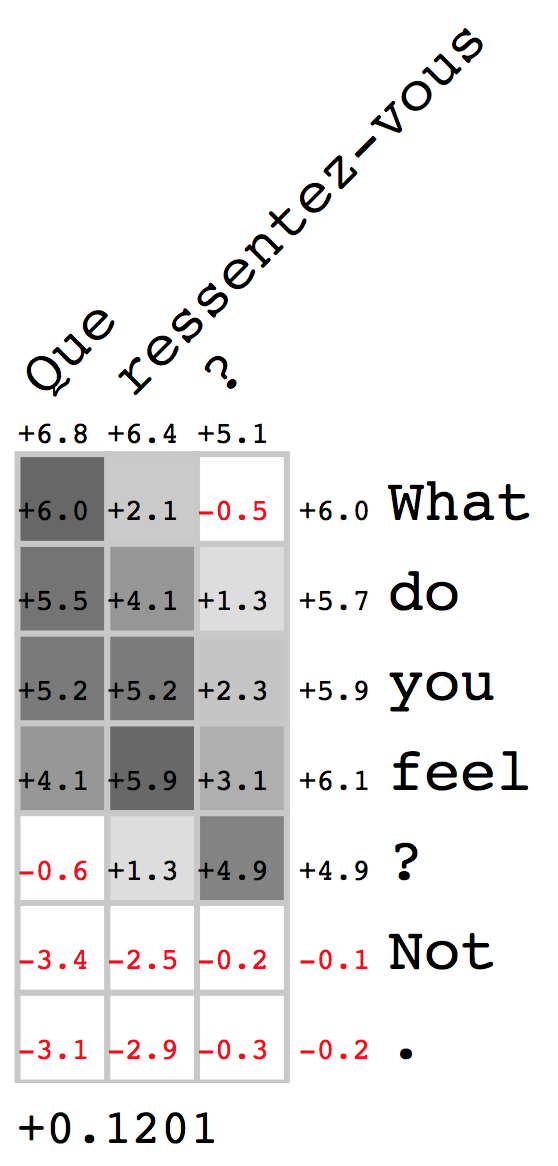
\includegraphics[width=0.35\linewidth]{feel}    
    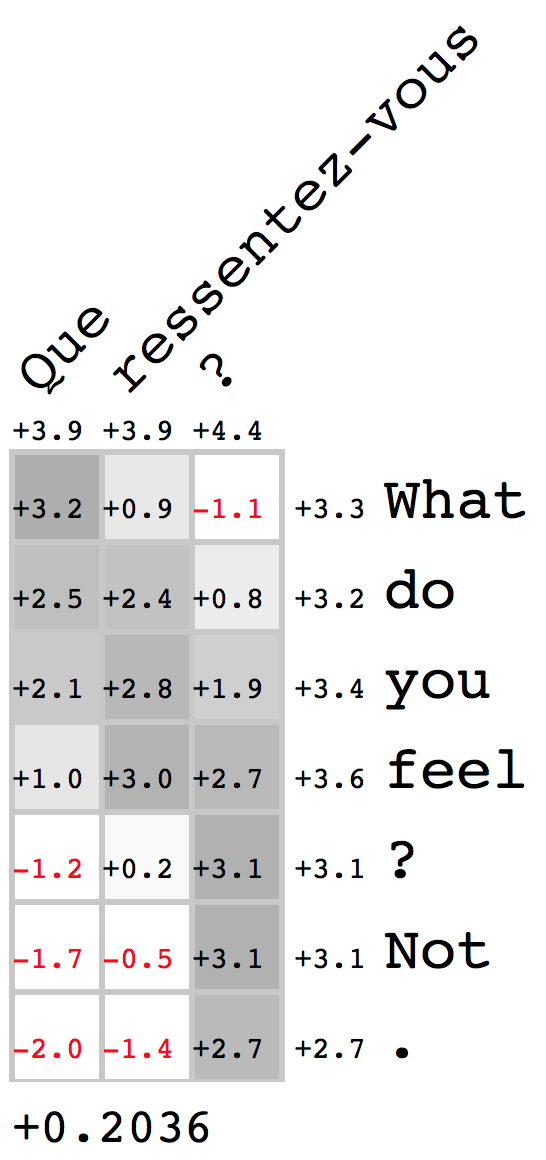
\includegraphics[width=0.35\linewidth]{feel_pu}    
\caption{Sentence pair with similarity scores produced by our model when trained over PU examples (right) and over PURI examples (left). Aggregation scores (Equation~\ref{aggregation}) are shown next to words. Matrices contain alignment scores. Sentence similarities (Equation~\ref{cosine})  shown below matrices.}
\label{matrix}
\end{figure}

Figure~\ref{matrix} illustrates the output of our network when trained using PU examples (right) and PURI examples (left).  
The former (right) fails to predict some word divergences, most likely because in training it never saw sentences mixing divergent and non-divergent words in the same example. 
%Furthermore, the latter (right) correctly assigns a lower similarity score to the sentence pair as both sentences do not convey the exact same meaning.

Table~\ref{results} shows BLEU results for our neural MT engine trained over different data configurations:
The entire\footnote{The original Paracrawl corpus contains more than $100$ million sentences. We reduced its size to $22.2$ millions using standard filtering techniques.} data (\texttt{all}); 
Most similar pairs after optimising equation~\ref{loss_semb} (\texttt{semb}); 
Most similar pairs after optimising equation~\ref{loss_wemb} (\texttt{wemb}); 
Finally, we apply the correction algorithm detailed in Section~\ref{correction} (\texttt{wemb+fix}).
Columns Ref and Fix indicate the number of original and corrected sentences (in millions) considered to train NMT.

\begin{table}[h!]
\small
\center
\begin{tabular}{lccl}
\hline
\bf Data & \bf Ref (M) & \bf Fix (M) & \bf Test (BLEU) \\ %MSLT & \bf NEWS \\
\hline
\multicolumn{3}{c}{\scriptsize{OpenSubtitles English-French}} \\
\texttt{all}                  & 27.2 & - & 42.18 \\
\texttt{semb}            & 18.0 & - & 41.95\\
\texttt{wemb}           & 15.5 & - & 43.12  ($+0.94$)\\
%\texttt{wemb}           & 21.5 & - & 42.56 \\
\texttt{wemb+fix}   & 15.5 & 2.5 & \\
\texttt{wemb}           & 18.0 & - & 43.19  ($+1.01$)\\
%\texttt{wemb+fix}   & 15.5 & 5.0 & \\
\hline
\multicolumn{3}{c}{\scriptsize{Paracrawl English-German}} \\
%\texttt{all}                  & 100.0 & 12.56 \\ 
\texttt{all}                  & 22.2 & - & 19.27 \\ 
\texttt{semb}            & 15.0 & - & \\
\texttt{wemb}           & 15.0 & - & 21.52 ($+2.25$)\\
%\texttt{wemb}           & 12.5 &   \\
%\texttt{wemb+fix}   & 12.5+2.5 & \\
\hline
\end{tabular}
\caption{BLEU scores obtained by neural MT using different subsets of the OpenSubtitles and Paracrawl corpora.}
\label{results}
\end{table}

Results for \texttt{wemb} clearly outperform the baseline \texttt{all} ($1^{st}$ rows) by about $+1.0$ and $+2.25$ BLEU ($3^{rd}$ rows). 
In contrast, \texttt{semb} does not improve over the baseline ($2^{nd}$ rows).
Regarding OpenSubtitles, an additional gain of $+X.X$ is found when fixing $2.5$ million sentences ($4^{th}$ row). 
The same $2.5$ million sentences did not show any improvement when added in their original form ($5^{th}$ row).

At this moment experiments showing correction results regarding Paracrawl  are not yet finished.

\section{Conclusions}
\label{conclusions}

We presented an unsupervised method based on deep neural networks for detecting translation divergences in parallel sentence pairs. 
Our model also predicts misaligned words that can then be filtered out allowing for reusing some divergent sentences.
We evaluated our model on two neural machine translation tasks, showing improvements when compared to training over the entire data set. 
%The method can be used on any parallel corpus without any manual annotation.

\section{Further Work}
\label{further}

%We plan to further evaluate divergence classification under different data noise levels. %and on additional language pairs. 
%as well as to measure the impact of using less noisy data when learning the similarity model
%We also would like to evaluate the impact of using less noisy (already filtered) data to learn the similarity model. 
%We would also like to use our model to predict other types of divergences 
We plan to use our model to predict sentence embeddings over monolingual corpora allowing to collect parallel pairs through vector similarity measures.
%We also plan to study the use of a neural network to predict divergent words, as a replacement for the algorithm detailed in Section~\ref{correction}.

%\section*{Acknowledgements}
%We are grateful to Jo\"el Legrand for his fruitful comments when building the neural divergence classifier.

\bibliography{biblio}
\bibliographystyle{acl_natbib_nourl}

\end{document}
